% ============================================================
%  Physics DPP — JEE Advanced 2026 | Class 12 | SolveFlow
% ============================================================
\documentclass[12pt,a4paper]{article}

\usepackage[a4paper, margin=2cm, top=2.5cm, bottom=2.5cm]{geometry}
\usepackage{xcolor}
\usepackage[most,breakable]{tcolorbox}
\usepackage{tikz}
\usepackage{amsmath,amssymb}
\usepackage{booktabs}
\usepackage{colortbl}
\usepackage{fancyhdr}
\usepackage{enumitem}
\usepackage{array}
\usepackage{multicol}
\usepackage{lastpage}

\usetikzlibrary{shapes.geometric,arrows.meta,positioning,calc,decorations.pathreplacing}

% ── Colours ──────────────────────────────────────────────────
\definecolor{accentcolor}{HTML}{0277BD}
\definecolor{accentlight}{HTML}{E3F2FD}
\definecolor{questionbg}{HTML}{E3F2FD}
\definecolor{questionborder}{HTML}{0277BD}
\definecolor{answerbg}{HTML}{E8F5E9}
\definecolor{answerborder}{HTML}{2E7D32}
\definecolor{notebg}{HTML}{FFF3E0}
\definecolor{noteborder}{HTML}{E65100}
\definecolor{rowA}{HTML}{F5F5F5}
\definecolor{rowB}{HTML}{FFFFFF}
\definecolor{darktext}{HTML}{212121}
\definecolor{mutedtext}{HTML}{757575}
\definecolor{coverdark}{HTML}{01579B}

% ── tcolorbox environments ────────────────────────────────────
\tcbuselibrary{skins,breakable,theorems}

\newtcolorbox{questionbox}[4]{
  enhanced, breakable,
  colback=questionbg, colframe=questionborder,
  boxrule=1pt, arc=4pt,
  title={\textbf{Q#1}\quad\textbar\quad\textit{#2}\hfill Marks:\ \textbf{#3}\quad\textbar\quad CO/BL:\ #4},
  fonttitle=\small\bfseries\color{white},
  colbacktitle=accentcolor,
  attach boxed title to top left={yshift=-2mm,xshift=4mm},
  boxed title style={arc=3pt,colframe=accentcolor},
  top=6mm
}

% ── Header / Footer ──────────────────────────────────────────
\pagestyle{fancy}
\fancyhf{}
\fancyhead[L]{\small\color{accentcolor}\textbf{Physics DPP \#1}}
\fancyhead[C]{\small\color{darktext}JEE Advanced 2026 \ $\cdot$\ Class 12}
\fancyhead[R]{\small\color{accentcolor}\textbf{SolveFlow}}
\fancyfoot[L]{\small\color{mutedtext}Topics: Electrostatics, Optics, Modern Physics, EMI, AC, Semiconductors}
\fancyfoot[C]{\small Page \thepage\ of \pageref{LastPage}}
\fancyfoot[R]{\small\color{mutedtext}Marks: +4 / $-$1}
\renewcommand{\headrulewidth}{0.6pt}
\renewcommand{\footrulewidth}{0.4pt}

% ─────────────────────────────────────────────────────────────
\begin{document}

% ═══════════════════════════════════════════════════════════
%  COVER PAGE
% ═══════════════════════════════════════════════════════════
\thispagestyle{empty}

\begin{tikzpicture}[remember picture, overlay]
  \fill[coverdark] (current page.north west) rectangle ([yshift=-4.2cm]current page.north east);
  \fill[accentcolor] ([yshift=-4.2cm]current page.north west) rectangle ([yshift=-4.7cm]current page.north east);
\end{tikzpicture}

\vspace*{0.4cm}
{\color{white}\fontsize{28}{34}\selectfont\bfseries\hspace{1cm}Physics}\\[4pt]
{\color{white!80!black}\fontsize{14}{18}\selectfont\hspace{1cm}Daily Practice Paper \#1\quad$\cdot$\quad JEE Advanced 2026\quad$\cdot$\quad Class 12}\\[2pt]
{\color{white!60!black}\fontsize{11}{14}\selectfont\hspace{1cm}SolveFlow\quad$\cdot$\quad Demo Paper}

\vspace{2.2cm}

% ── Summary table ────────────────────────────────────────────
\begin{center}
\renewcommand{\arraystretch}{1.4}
\begin{tabular}{>{\bfseries\color{accentcolor}}p{5cm} p{8cm}}
\toprule
\rowcolor{rowA} Field & Value \\
\midrule
\rowcolor{rowB} Subject & Physics \\
\rowcolor{rowA} Total Questions & 10 \\
\rowcolor{rowB} Total Marks & 40 \\
\rowcolor{rowA} Negative Marking & $-1$ per wrong answer \\
\rowcolor{rowB} Time Suggested & 30 minutes \\
\rowcolor{rowA} Syllabus & Class 12 — Electrostatics, Current Electricity, \\
         & EMI, Optics, Modern Physics, Semiconductors \\
\bottomrule
\end{tabular}
\end{center}

\vspace{0.6cm}

% ── CO Mapping table ─────────────────────────────────────────
\begin{center}
{\color{accentcolor}\large\bfseries CO \& Bloom's Level Mapping}\\[6pt]
\renewcommand{\arraystretch}{1.35}
\begin{tabular}{>{\centering\arraybackslash}p{1.2cm}
                >{\raggedright\arraybackslash}p{4.5cm}
                >{\centering\arraybackslash}p{1.5cm}
                >{\raggedright\arraybackslash}p{4.5cm}}
\toprule
\rowcolor{accentcolor}
\color{white}\bfseries Q No. & \color{white}\bfseries Topic & \color{white}\bfseries CO & \color{white}\bfseries Bloom's Level \\
\midrule
\rowcolor{rowB} 1 & Electrostatics — Point Charges & CO1 & L3 — Apply \\
\rowcolor{rowA} 2 & Current Electricity — Wheatstone Bridge & CO1 & L3 — Apply \\
\rowcolor{rowB} 3 & Magnetic Effects of Current & CO2 & L4 — Analyse \\
\rowcolor{rowA} 4 & Electromagnetic Induction & CO2 & L3 — Apply \\
\rowcolor{rowB} 5 & Alternating Current — Resonance & CO2 & L3 — Apply \\
\rowcolor{rowA} 6 & Ray Optics — Lens Formula & CO3 & L3 — Apply \\
\rowcolor{rowB} 7 & Wave Optics — YDSE & CO3 & L3 — Apply \\
\rowcolor{rowA} 8 & Dual Nature — de Broglie & CO4 & L2 — Understand \\
\rowcolor{rowB} 9 & Atoms \& Nuclei — Hydrogen Spectrum & CO4 & L3 — Apply \\
\rowcolor{rowA} 10 & Semiconductors — p-n Junction & CO5 & L2 — Understand \\
\bottomrule
\end{tabular}
\end{center}

\vspace{0.6cm}

\begin{tcolorbox}[colback=accentlight,colframe=accentcolor,arc=4pt,boxrule=1pt,
  title={\bfseries\color{white} Instructions},colbacktitle=accentcolor]
\begin{itemize}[noitemsep,topsep=2pt]
  \item Each question carries \textbf{4 marks} for a correct answer.
  \item \textbf{$-1$ mark} is deducted for each incorrect answer.
  \item No marks are deducted for unattempted questions.
  \item Use of calculator is \textbf{not} permitted.
  \item Write answers clearly in the response sheet.
\end{itemize}
\end{tcolorbox}

\newpage

% ═══════════════════════════════════════════════════════════
%  QUESTIONS
% ═══════════════════════════════════════════════════════════

% ── Q1 ───────────────────────────────────────────────────────
\begin{questionbox}{1}{Electrostatics}{4}{CO1 / L3}
Two conducting spheres of radii $r_1$ and $r_2$ are charged to the \textbf{same surface charge density}
$\sigma$. The ratio of their electric potentials $\dfrac{V_1}{V_2}$ is:

\begin{enumerate}[label=(\Alph*), itemsep=4pt, topsep=6pt]
  \item $\dfrac{r_2}{r_1}$
  \item $\dfrac{r_1}{r_2}$
  \item $\left(\dfrac{r_1}{r_2}\right)^2$
  \item $1$
\end{enumerate}
\end{questionbox}




% ── Q2 ───────────────────────────────────────────────────────
\begin{questionbox}{2}{Current Electricity — Wheatstone Bridge}{4}{CO1 / L3}
In a balanced Wheatstone bridge $P/Q = R/S$, with $P = 10\,\Omega$, $Q = 5\,\Omega$.
The value of $S$ at balance when $R = 20\,\Omega$ is:

\begin{center}
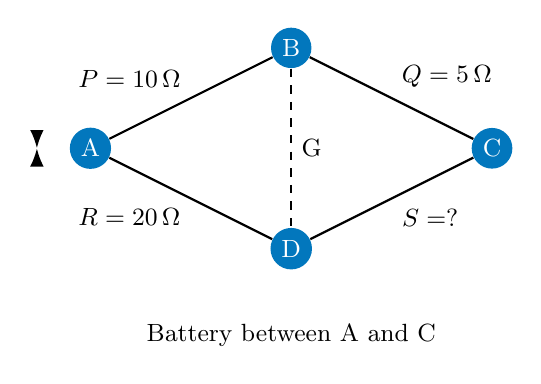
\begin{tikzpicture}[scale=0.85, every node/.style={font=\small}]
  % Nodes
  \node[circle,fill=accentcolor,text=white,inner sep=2pt] (A) at (0,0)   {A};
  \node[circle,fill=accentcolor,text=white,inner sep=2pt] (B) at (3,1.5) {B};
  \node[circle,fill=accentcolor,text=white,inner sep=2pt] (C) at (6,0)   {C};
  \node[circle,fill=accentcolor,text=white,inner sep=2pt] (D) at (3,-1.5){D};
  % Arms
  \draw[thick] (A)--(B) node[midway,above left]{$P=10\,\Omega$};
  \draw[thick] (B)--(C) node[midway,above right]{$Q=5\,\Omega$};
  \draw[thick] (A)--(D) node[midway,below left]{$R=20\,\Omega$};
  \draw[thick] (D)--(C) node[midway,below right]{$S=?$};
  % Galvanometer
  \draw[thick,dashed] (B)--(D) node[midway,right]{G};
  % Battery
  \draw[thick,{Latex}-{Latex}] (-0.8,0)--(-0.8,0) node{};
  \node at (3,-2.8) {Battery between A and C};
\end{tikzpicture}
\end{center}

\begin{enumerate}[label=(\Alph*), itemsep=4pt, topsep=6pt]
  \item $8\,\Omega$
  \item $10\,\Omega$
  \item $12\,\Omega$
  \item $6\,\Omega$
\end{enumerate}
\end{questionbox}




% ── Q3 ───────────────────────────────────────────────────────
\begin{questionbox}{3}{Magnetic Effects of Current}{4}{CO2 / L4}
A proton moves with speed $v$ in a uniform magnetic field $B$.
The angle between $\vec{v}$ and $\vec{B}$ is $30^\circ$.
The radius of the \textbf{circular component} of its helical path is:

\begin{enumerate}[label=(\Alph*), itemsep=4pt, topsep=6pt]
  \item $\dfrac{mv}{2qB}$
  \item $\dfrac{mv\sin 30^\circ}{qB}$
  \item $\dfrac{mv\cos 30^\circ}{qB}$
  \item $\dfrac{mv}{qB\sin 30^\circ}$
\end{enumerate}
\end{questionbox}




% ── Q4 ───────────────────────────────────────────────────────
\begin{questionbox}{4}{Electromagnetic Induction}{4}{CO2 / L3}
A square loop of side $10\,\text{cm}$ is placed in a uniform magnetic field
$B = 0.5\,\text{T}$ perpendicular to its plane. The loop is pulled completely
out of the field in $0.1\,\text{s}$. The induced EMF is:

\begin{enumerate}[label=(\Alph*), itemsep=4pt, topsep=6pt]
  \item $0.05\,\text{V}$
  \item $0.5\,\text{V}$
  \item $0.005\,\text{V}$
  \item $5\,\text{V}$
\end{enumerate}
\end{questionbox}




% ── Q5 ───────────────────────────────────────────────────────
\begin{questionbox}{5}{Alternating Current — Resonance}{4}{CO2 / L3}
A series RLC circuit has $R = 100\,\Omega$, $L = 1\,\text{H}$, $C = 100\,\mu\text{F}$.
The resonant frequency $f_0$ is approximately:

\begin{enumerate}[label=(\Alph*), itemsep=4pt, topsep=6pt]
  \item $15.9\,\text{Hz}$
  \item $50\,\text{Hz}$
  \item $100\,\text{Hz}$
  \item $31.8\,\text{Hz}$
\end{enumerate}
\end{questionbox}




% ── Q6 ───────────────────────────────────────────────────────
\begin{questionbox}{6}{Ray Optics — Convex Lens}{4}{CO3 / L3}
A convex lens of focal length $f = 20\,\text{cm}$ forms a real image of an object
placed $30\,\text{cm}$ from the lens. The image distance $v$ is:

\begin{center}
\begin{tikzpicture}[scale=0.75]
  % Principal axis
  \draw[->] (-4,0)--(5,0) node[right]{\small Principal axis};
  % Lens
  \draw[thick,blue!70!black] (0,-1.8)--(0,1.8);
  \draw[thick,blue!70!black] (0,1.8) arc(90:75:7);
  \draw[thick,blue!70!black] (0,-1.8) arc(270:285:7);
  % Object
  \draw[->,thick,red!70!black] (-3,0)--(-3,1.2) node[above]{\small O};
  % Image
  \draw[->,thick,green!50!black] (4,0)--(4,-2.4) node[below]{\small I};
  % Labels
  \node[below] at (-3,-0.1) {\small $u=-30$\,cm};
  \node[below] at (4,-0.1)  {\small $v=?$};
  \node[below] at (0,-2.1)  {\small $f=20$\,cm};
  % F points
  \filldraw (2,0) circle(1.5pt) node[above]{\small F};
  \filldraw (-2,0) circle(1.5pt) node[above]{\small F$'$};
\end{tikzpicture}
\end{center}

\begin{enumerate}[label=(\Alph*), itemsep=4pt, topsep=6pt]
  \item $60\,\text{cm}$
  \item $12\,\text{cm}$
  \item $-60\,\text{cm}$
  \item $-12\,\text{cm}$
\end{enumerate}
\end{questionbox}




% ── Q7 ───────────────────────────────────────────────────────
\begin{questionbox}{7}{Wave Optics — Young's Double Slit}{4}{CO3 / L3}
In YDSE, slit separation $d = 0.5\,\text{mm}$, screen distance $D = 1\,\text{m}$,
wavelength $\lambda = 600\,\text{nm}$. The fringe width $\beta$ is:

\begin{enumerate}[label=(\Alph*), itemsep=4pt, topsep=6pt]
  \item $1.2\,\text{mm}$
  \item $0.6\,\text{mm}$
  \item $1.0\,\text{mm}$
  \item $2.4\,\text{mm}$
\end{enumerate}
\end{questionbox}




% ── Q8 ───────────────────────────────────────────────────────
\begin{questionbox}{8}{Dual Nature of Matter}{4}{CO4 / L2}
The de Broglie wavelength of an electron accelerated through $V = 100\,\text{V}$ is:

\begin{enumerate}[label=(\Alph*), itemsep=4pt, topsep=6pt]
  \item $1.23\,\text{\AA}$
  \item $0.123\,\text{nm}$
  \item $12.3\,\text{\AA}$
  \item Both (A) and (B) are correct
\end{enumerate}
\end{questionbox}




% ── Q9 ───────────────────────────────────────────────────────
\begin{questionbox}{9}{Atoms \& Nuclei — Hydrogen Spectrum}{4}{CO4 / L3}
An electron in a hydrogen atom transitions from $n = 3$ to $n = 2$
(Balmer series). The wavelength of the emitted radiation is approximately:

\begin{enumerate}[label=(\Alph*), itemsep=4pt, topsep=6pt]
  \item $656\,\text{nm}$
  \item $121\,\text{nm}$
  \item $486\,\text{nm}$
  \item $365\,\text{nm}$
\end{enumerate}
\end{questionbox}




% ── Q10 ──────────────────────────────────────────────────────
\begin{questionbox}{10}{Semiconductors — p-n Junction}{4}{CO5 / L2}
In a p-n junction diode under \textbf{forward bias}, the width of the depletion layer:

\begin{enumerate}[label=(\Alph*), itemsep=4pt, topsep=6pt]
  \item Increases
  \item Decreases
  \item Remains unchanged
  \item First increases then decreases
\end{enumerate}
\end{questionbox}


\label{LastPage}
\end{document}
